\chapter{Ayrıklaştırma}
Türevin geometrik yorumu 
\begin{equation}
    \frac{dy(t)}{dt}\approx\frac{\Delta y}{\Delta t}
\end{equation}
olmak üzere
\begin{equation}
\begin{split}
    \frac{dy(t)}{dt}&\approx\frac{\Delta y}{\Delta t}\\
    &\approx\frac{y((k+1)T)-y(kT)}{(k+1)T-kT}\\
    &\approx\frac{y((k+1)T)-y(kT)}{T}
\end{split}
\end{equation}
elde edilir. Ayrık bir sinyalin türevi ardışık değerler farkının örnekleme zamanına oranı ile hesaplanabilmektedir. Örneğin, $y(kT)=\sin(kT)$ ve $T=0.1$ olmak üzere
\begin{equation}
    \frac{y((k+1)T)-y(kT)}{T}=10(\sin((k+1)0.1)-\sin(0.1k))
\end{equation}
ve dolayısıyla
\begin{equation}
\begin{split}
    \{10\sin(0.1),10(\sin(0.2)-\sin(0.1)),10(\sin(0.3)-\sin(0.2)),\cdots\}\\
    \{0.9983,0.9884, 0.9685,\cdots\}
\end{split}
\end{equation}
elde edilir. $y(kT)=\sin(kT)$ sinyalinin türevinin $\frac{d\sin(t)}{dt}=\cos(t)$ olduğu bilindiğinden
\begin{equation}
    \begin{split}
        \{cos(0.1),cos(0.2),cos(0.3),\cdots\}\\
        \{ 0.9950,0.9801,0.9553,\cdots\}
    \end{split}
\end{equation}
elde edilir ve ayrık türev ile benzer değerler olduğu görülmektedir. Bu yaklaşıklığın türeve yakınsaması için örnekleme zamanı $T$ daha küçük seçilmelidir. 
\begin{equation}
    \frac{dq(t)}{dt}=x
\end{equation}
olmak üzere
\begin{equation}
\begin{split}
    \frac{dq(t)}{dt}&=x\\
    dq(t)&=xdt\\
    \int dq(t)&=\int xdt\\
    q(t)&=\int xdt
\end{split}
\end{equation}
elde edilir. Buradan hareketle,
\begin{equation}
    \begin{split}
        \frac{\Delta q}{\Delta t}&=x\\
        \frac{q((k+1)T)-q(kT)}{(k+1)T-kT}&=x\\
        \frac{q((k+1)T)-q(kT)}{T}&=x\\
        q((k+1)T)-q(kT)&=xT\\
        q((k+1)T)&=q(kT)+xT
    \end{split}
\end{equation}
ifadesi bulunur. Ayrık zamanda integral birikimli toplama karşılık gelmektedir. Bu karşılıklar Zero Order Hold(ZOH) ile elde edilmiştir. ZOH örnekleme zamanı boyunca değerlerin sabit olduğu varsayımına dayanmaktadır. Bu durum
\begin{equation}
    x(t)=x(kT),\quad kT\leq t\leq (k+1)T
\end{equation}
ile ifade edilebilir. ZOH için transfer fonksiyonu elde etmek amacıyla girişe $\delta(t)$ birim darbe fonksiyonu uygulanırsa çıkışında $u(t)-u(t-T)$ elde edilir. Bu durumda S tanım bölgesinde çıkış ifadesi
\begin{equation}
\begin{split}
    \mathcal{L}\{u(t)-u(t-T)\}&=\mathcal{L}\{u(t)\}-\mathcal{L}\{u(t-T)\}\\
    &=\mathcal{L}\{u(t)\}-e^{-sT}\mathcal{L}\{u(t)\}\\
    &=\frac{1}{s}-e^{-sT}\frac{1}{s}\\
    &=(1-e^{-sT})\frac{1}{s}
\end{split}
\end{equation}
şeklindedir. ZOH transfer fonksiyonu ile bir $G(s)$ sistemi birlikte Z dönüşümü yapılmalıdır. Örneğin,
\begin{equation}
    G(s)=\frac{1}{s+1}
    \label{eqn:ornek_sistem}
\end{equation}
sistemi ayrıklaştırılmak istensin. Bu durumda $G_{ZOH}(s)G(s)$ ayrıklaştırılmalıdır. Bu sebeple,
\begin{equation}
    L(s)=G_{ZOH}(s)G(s)=\frac{1-e^{-sT}}{s(s+1)}
\end{equation}
ifadesi Z tanım bölgesine
\begin{equation}
\begin{split}
    \mathcal{Z}\{L(s)\}&=\mathcal{Z}\left\{\frac{1-e^{-sT}}{s(s+1)}\right\}\\
    &=\mathcal{Z}\{1-e^{-sT}\} \mathcal{Z}\left\{\frac{1}{s(s+1)} \right\}\\
    &=(1-z^{-1}) \left(\mathcal{Z}\left\{\frac{1}{s}-\frac{1}{s+1} \right\}\right)\\
    &=\left(1-\frac{1}{z}\right) \left(\mathcal{Z}\left\{\frac{1}{s}\right\}-\mathcal{Z}\left\{\frac{1}{s+1} \right\}\right)\\
    &=\frac{z-1}{z} \left(\frac{z}{z-1}-\frac{z}{z-e^{-1}}\right)\\
    &=\left(1-\frac{z-1}{z-e^{-1}}\right)\\
    &=\frac{1-e^{-1}}{z-e^{-1}}
\end{split}\label{eqn:ornek_sistem_zoh}
\end{equation}
olarak dönüştürülür.

First Order Hold(FOH) yöntemi ise
\begin{equation}
    x(t)=x(kT)+\frac{t-kT}{T}(x((k+1)T)-x(kT)),\quad kT\leq t\leq (k+1)T
\end{equation}
olarak tanımlanır. Eşitliğin sağ tarafı $t=kT$ için $x(kT)$, $t=(k+0.5)T$ için 
\begin{equation}
\begin{split}
    x(t)&=x(kT)+\frac{t-kT}{T}(x((k+1)T)-x(kT)),\quad kT\leq t\leq (k+1)T\\
    &=x(kT)+\frac{kT+0.5T-kT}{T}(x((k+1)T)-x(kT))\\
    &=x(kT)+0.5(x((k+1)T)-x(kT))\\
    &=x(kT)+0.5x((k+1)T)-0.5x(kT)\\
    &=0.5x((k+1)T)+0.5x(kT)
\end{split}
\end{equation}
ve $t=(k+1)T$ için ise 
\begin{equation}
    \begin{split}
        x(t)&=x(kT)+\frac{t-kT}{T}(x((k+1)T)-x(kT)),\quad kT\leq t\leq (k+1)T\\
        x(t)&=x(kT)+\frac{(k+1)T-kT}{T}(x((k+1)T)-x(kT))\\
        x(t)&=x(kT)+x((k+1)T)-x(kT)\\
        x(t)&=x((k+1)T)
    \end{split}
\end{equation}
olarak elde edilir. Görüldüğü üzere ZOH yönteminin aksine $T$ süre boyunca değerler değişmektedir. FOH için birim darbe yanıtı
\begin{equation}
    x(t)=\begin{cases}
        t+\frac{1}{T} & 0\leq t\leq \frac{1}{T}\\
        -t+\frac{1}{T} & \frac{1}{T}\leq t\leq \frac{2}{T}\\
        0 & t>\frac{2}{T}
    \end{cases}
\end{equation}
ve işlem kolaylığı açısından $T=1$ alınırsa 
\begin{equation}
    x(t)=(1-t)u(2-t)+2tu(1-t)
\end{equation}
şeklindedir. S dönüşümü sonucu
\begin{equation}
\begin{split}
    \mathcal{L}\{x(t)\}&=\mathcal{L}\{(1-t)u(2-t)\}+\mathcal{L}\{2tu(1-t)\}\\
    &=\mathcal{L}\{(1-t)(1-u(t-2))\}+\mathcal{L}\{2t(1-u(t-1))\}\\
    &=\mathcal{L}\{(1-t)\}-\mathcal{L}\{(1-t)u(t-2)\}+\mathcal{L}\{2t\}-\mathcal{L}\{2tu(t-1)\}\\
    &=\mathcal{L}\{(1+t)\}+\mathcal{L}\{(t-1)u(t-2)\}-\mathcal{L}\{2tu(t-1)\}\\
    &=\mathcal{L}\{(1+t)\}+\mathcal{L}\{(t-1)u(t-2)\}-\mathcal{L}\{(2t-2+2)u(t-1)\}\\
    &=\mathcal{L}\{(1+t)\}+\mathcal{L}\{(t-1-1+1)u(t-2)\}-\mathcal{L}\{(2t-2+2)u(t-1)\}\\
    &=\mathcal{L}\{(1+t)\}+\mathcal{L}\{(t-2)u(t-2)+u(t-2)\}-\mathcal{L}\{(2t-2)u(t-1)+2u(t-1)\}\\
    &=\frac{1}{s}+\frac{1}{s^2}+\frac{e^{-2s}}{s^2}+\frac{e^{-2s}}{s}-2\frac{e^{-s}}{s^2}-\frac{2e^{-s}}{s}\\
    &=\frac{1-2e^{-s}+e^{-2s}}{s}+\frac{1-2e^{-s}+e^{-2s}}{s^2}\\
    &=\frac{(1-e^{-s})^2}{s}+\frac{(1-e^{-s})^2}{s^2}\\
    &=\frac{(1-e^{-s})^2}{s^2}(s+1)\\
\end{split}
\end{equation}
elde edilir. FOH için transfer fonksiyonu
\begin{equation}
    \begin{split}
        G_{FOH}(s)&=\frac{(1-e^{-s})^2}{T^2s^2}\frac{Ts+1}{T}\\
        &=G_{ZOH}^2(s)\frac{Ts+1}{T}
\end{split}
\end{equation}
şeklindedir. Örneğin daha önce Denklem~\ref{eqn:ornek_sistem} ile verilen sistemi FOH yöntemi ve yine aynı örnekleme zamanı ile ayrıklaştırmak gerekirse
\begin{equation}
\begin{split}
    L(s)&=\frac{1}{s+1}G_{FOH}(s)\\
    &=\frac{1}{s+1}\frac{(1-e^{-s})^2}{T^2s^2}\frac{Ts+1}{T}\\
    &=\frac{1}{s+1}\frac{(1-e^{-s})^2}{s^2}(s+1)\\
    &=\frac{(1-e^{-s})^2}{s^2}
\end{split}
\end{equation}
ifadesi Z dönüşümüne tabi tutulmalıdır. Dolayısıyla,
\begin{equation}
    \begin{split}
        G(z)&=\mathcal{Z}\left\{\frac{(1-e^{-s})^2}{s^2}\right\}\\
        &=\mathcal{Z}\{(1-e^{-s})^2\}\mathcal{Z}\left\{\frac{1}{s^2}\right\}\\
        &=\left(1-z^{-1}\right)^2\frac{Tz}{(z-1)^2}\\
        &=\left(\frac{z-1}{z}\right)^2\frac{z}{(z-1)^2}\\
        &=\frac{1}{z}
    \end{split}\label{eqn:ornek_sistem_foh}
\end{equation}
elde edilir. Görüldüğü üzere, birim gecikme elde edilmiştir.

\begin{enumerate}
    \item $x(t)=sin(t)$ fonksiyonunun türevini hesaplayıp çiziniz.
    \begin{lstlisting}[style=Matlab-editor]
    t=0:0.1:10;
    xt=sin(t);
    dxt=zeros(size(t));
    T=t(2)-t(1);
    for i=2:length(t)
        dxt(i)=(xt(i)-xt(i-1))/T;
    end
    figure(1);clf;hold on;grid on;xlabel("Zaman(s)");ylabel("x(t)");title("sin(t) ve turevi");
    plot(t,xt,'k','LineWidth',2);
    plot(t,dxt,'r','LineWidth',2);
    \end{lstlisting}
    Şekil~\ref{fig:lec2_plot1}'de $sin(t)$ ve türevi gösterilmiştir.
    \begin{figure}[!htb]
        \centering
        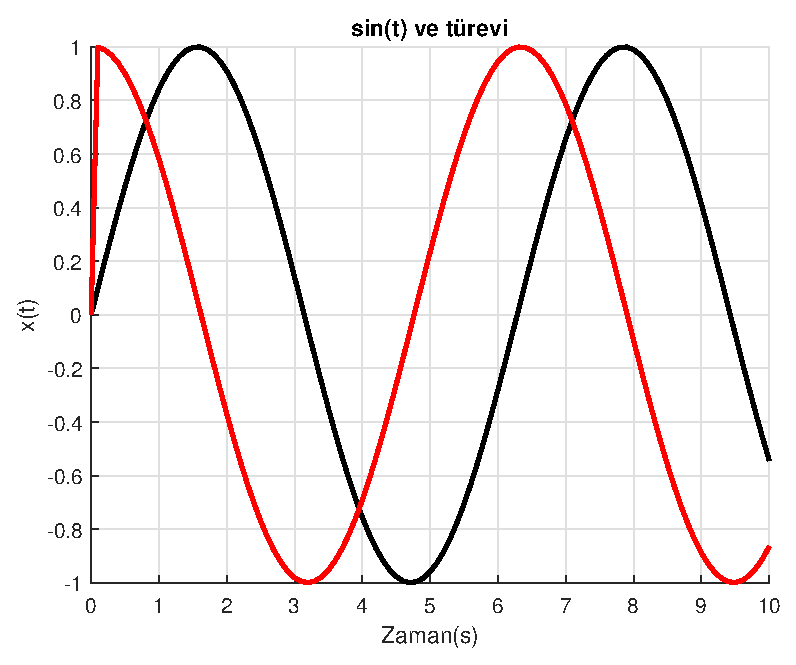
\includegraphics[width=0.5\textwidth]{img/lec2_plot1}
        \caption{$sin(t)$ ve türevinin karşılaştırılması($T=0.1$)}
        \label{fig:lec2_plot1}
    \end{figure}

    Şekil~\ref{fig:lec2_plot2}'de daha düşük bir örnekleme zamanı seçilmiştir ve bu sebeple gerek sinyal gerekse türevi düşük kalitededir.
    \begin{figure}[!htb]
        \centering
        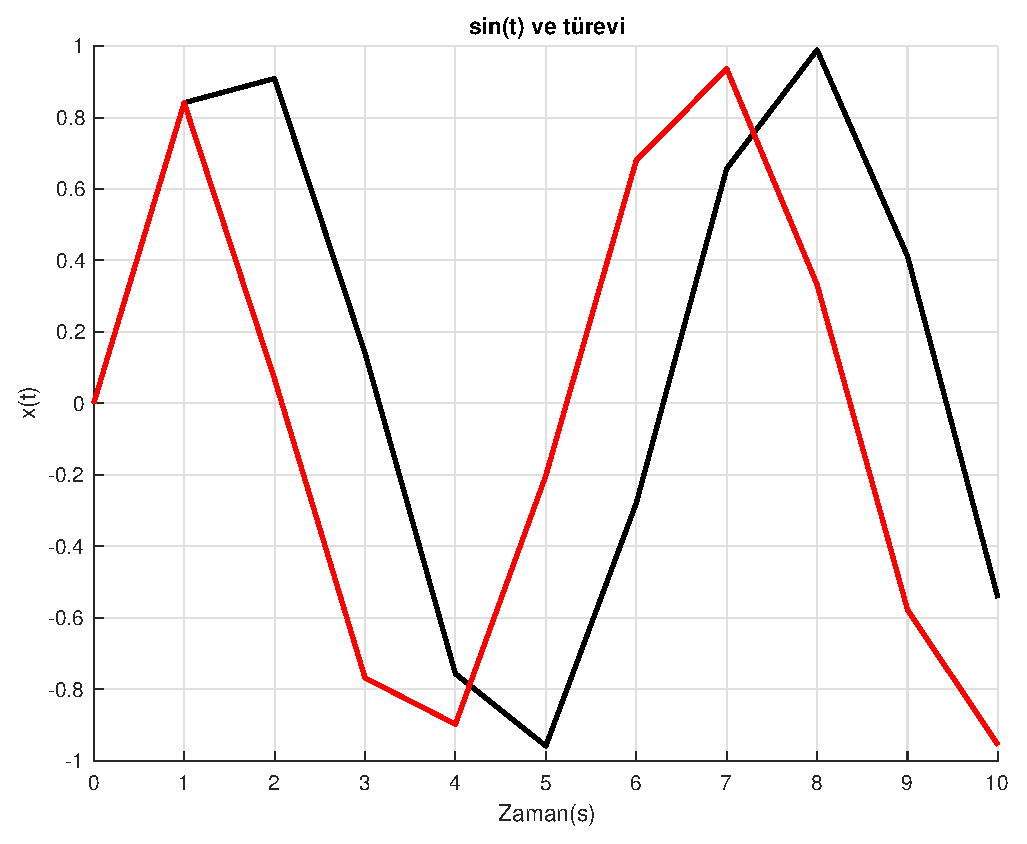
\includegraphics[width=0.5\textwidth]{img/lec2_plot2}
        \caption{$sin(t)$ ve türevinin karşılaştırılması($T=1$)}
        \label{fig:lec2_plot2}
    \end{figure}
    \item $x(t)=e^{-t}$ sinyalinin integralini hesaplayınız ve çizdiriniz.
    \begin{lstlisting}[style=Matlab-editor]
    t=0:1:10;
    xt=exp(-t);
    q=zeros(size(t));
    T=t(2)-t(1);
    for i=2:length(t)
        q(i)=q(i-1)+xt(i-1)*T;
    end
    figure(1);clf;hold on;grid on;xlabel("Zaman(s)");ylabel("x(t)");title("sin(t) ve integrali");
    plot(t,xt,'k','LineWidth',2);
    plot(t,q,'r','LineWidth',2);
    \end{lstlisting}
    Şekil~\ref{fig:lec2_plot3}'de integral çizdirilmiştir.
    \begin{figure}[!htb]
        \centering
        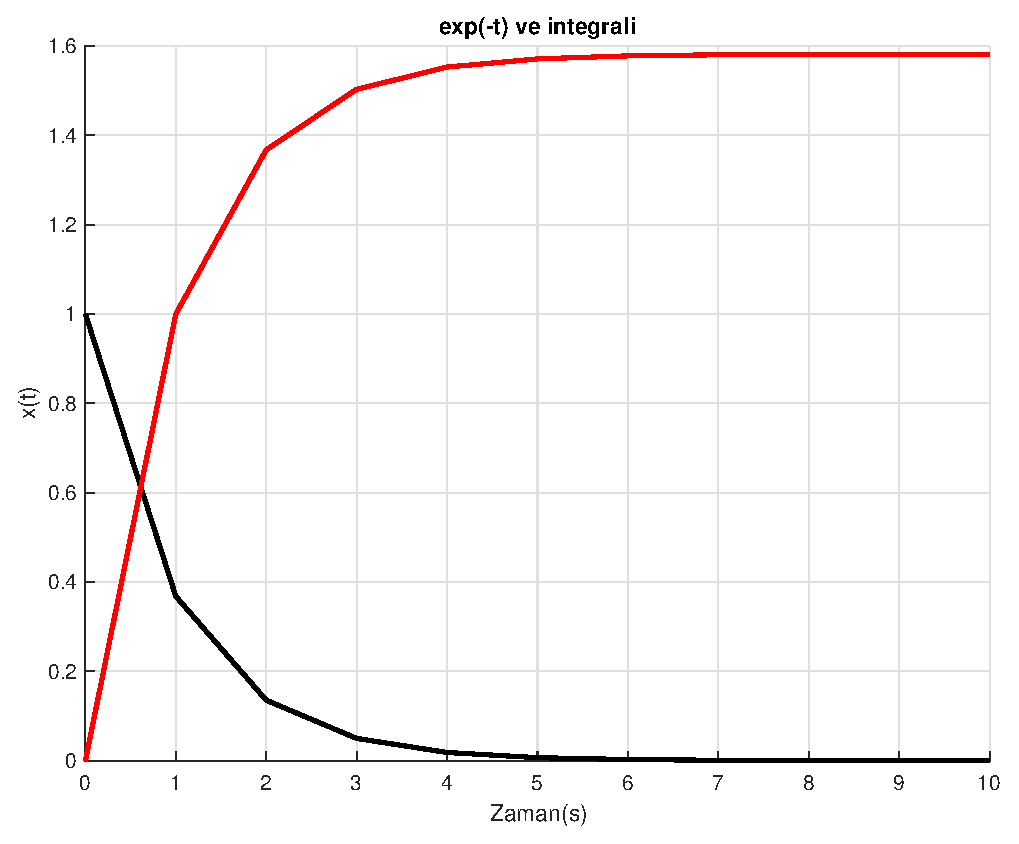
\includegraphics[width=0.5\textwidth]{img/lec2_plot3}
        \caption{$sin(t)$ ve integralinin karşılaştırılması($T=1$)}
        \label{fig:lec2_plot3}
    \end{figure}
    \item ZOH yöntemini kullanarak $T=1$ olmak üzere $x(kT)=1$ sinyalini veri tutucunu çıkışını çizdiriniz.
    \begin{lstlisting}[style=Matlab-editor]
    T=1;
    t=0:T:3;
    xt=[1,2,-1,3];
    
    tnew=0:0.01:4;
    yt=zeros(size(tnew));
    for i=1:length(t)
        for j=1:100
            yt(100*(i-1)+j)=xt(i);
        end
    end
    figure(1);clf;hold on;grid on;xlabel("Zaman(s)");ylabel("x(t)");title("ZOH ornegi");
    stem(t,xt,'k','LineWidth',2);
    plot(tnew,yt,'r','LineWidth',2);
    \end{lstlisting}
    Şekil~\ref{fig:lec2_plot4}'de ZOH işleminin sonucu gösterilmiştir.
    \begin{figure}[!htb]
        \centering
        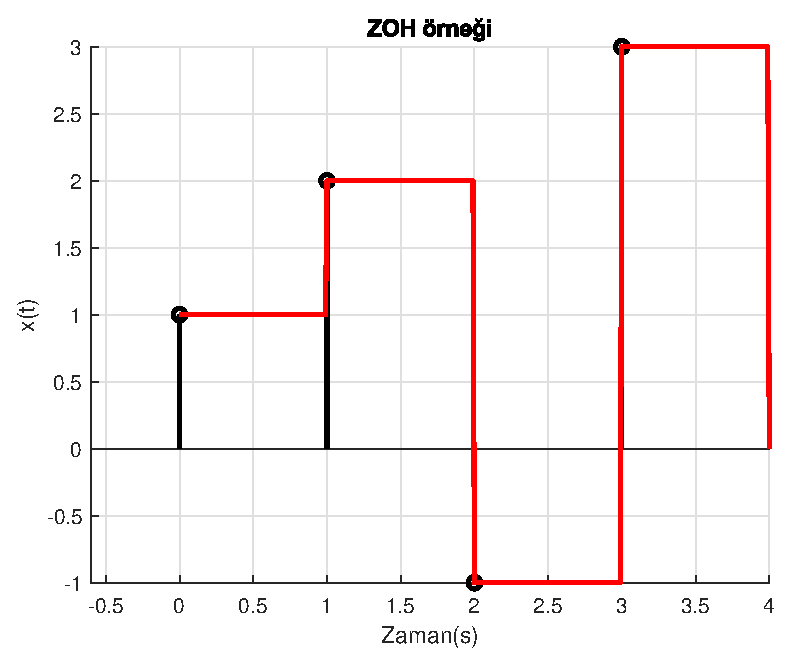
\includegraphics[width=0.5\textwidth]{img/lec2_plot4}
        \caption{ZOH örneği}
        \label{fig:lec2_plot4}
    \end{figure}
    \item FOH yöntemini kullanarak $T=1$ olmak üzere $x(kT)=1$ sinyalini veri tutucunu çıkışını çizdiriniz.
    \begin{lstlisting}[style=Matlab-editor]
    T=1;
    t=0:T:3;
    xt=[1,2,-1,3];
    
    tnew=0:0.01:4;
    yt=zeros(size(tnew));
    for i=1:length(t)-1
        for j=1:100
            yt(100*(i-1)+j)=xt(i)+0.01*j*(xt(i+1)-xt(i));
        end
    end
    figure(1);clf;hold on;grid on;xlabel("Zaman(s)");ylabel("x(t)");title("ZOH ornegi");
    stem(t,xt,'k','LineWidth',2);
    plot(tnew,yt,'r','LineWidth',2);
    \end{lstlisting}
    Şekil~\ref{fig:lec2_plot5}'de FOH işleminin sonucu gösterilmiştir.
    \begin{figure}[!htb]
        \centering
        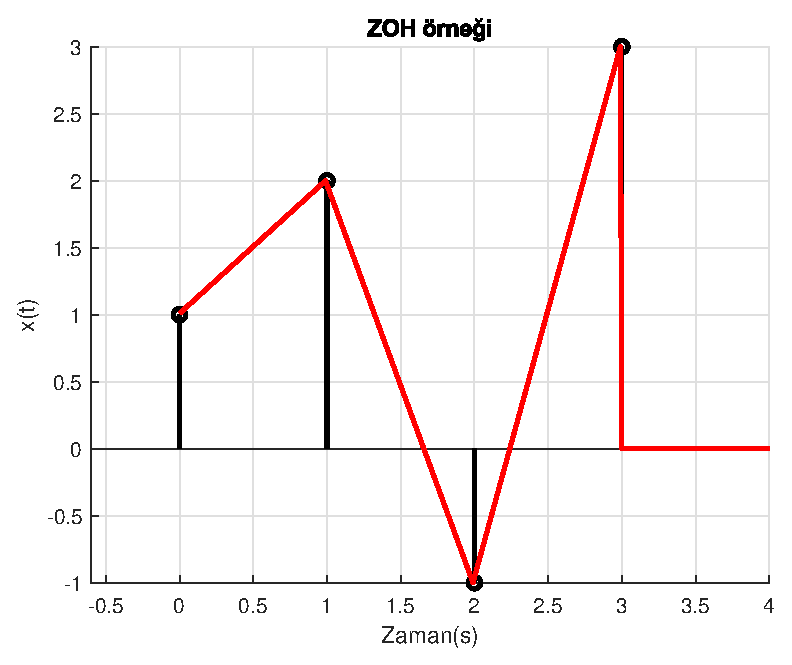
\includegraphics[width=0.5\textwidth]{img/lec2_plot5}
        \caption{FOH örneği}
        \label{fig:lec2_plot5}
    \end{figure}
\end{enumerate}